\documentclass[a4paper, 14pt]{extarticle}

\usepackage[T2A]{fontenc}
\usepackage[utf8]{inputenc}
\usepackage[russian]{babel}

\usepackage{graphicx}
\usepackage{hyperref}

\begin{document}
\setlength{\emergencystretch}{1em}
\begin{titlepage}
  \centering

  Общероссийская общественно-государственная организация 
  ``Всероссийское общество изобретателей и рационализаторов'' (ВОИР)                        

  \vfill

  {\Large\bfseries ПОЛЁТНОЕ ЗАДАНИЕ\par}
  \vspace{1cm}
  {\large RoboTrio (БАС)\par}
  
  \vfill

  \begin{flushright}
    Разработал: AIRES
  \end{flushright}

  \vfill
  
  Новосибирск\\
  \the\year
\end{titlepage}

\tableofcontents

\newpage

\section{Введение}
Настоящее полётное задание разработано в рамках учебно"=демонстрационной миссии беспилотной авицианной системы (БАС, дрона) в проекте ``RoboTrio''. Оно устанавливает сценарий полёта дрона, а также регламентирует его действия в случае несшатных или аварийных ситуаций.

\textbf{Основная цель} дрона в рамках миссии заключается в переносе грузов-моделей с установчного пункта (``склад'') на заданный заранее иной пункт, между которыми расположено высотное физическое препятствие в виде модели горы. Миссия должна производится в режиме самостоятельного полёта с принятием решений на основе методов компьютерного зрения и анализа телеметрии. 

В рамках техники безопасности оборудования и персонала проекта предусматривается наличие источника ручного управления полётом.

\section{Описание элементов управления}
\begin{figure}[h]
  \centering
  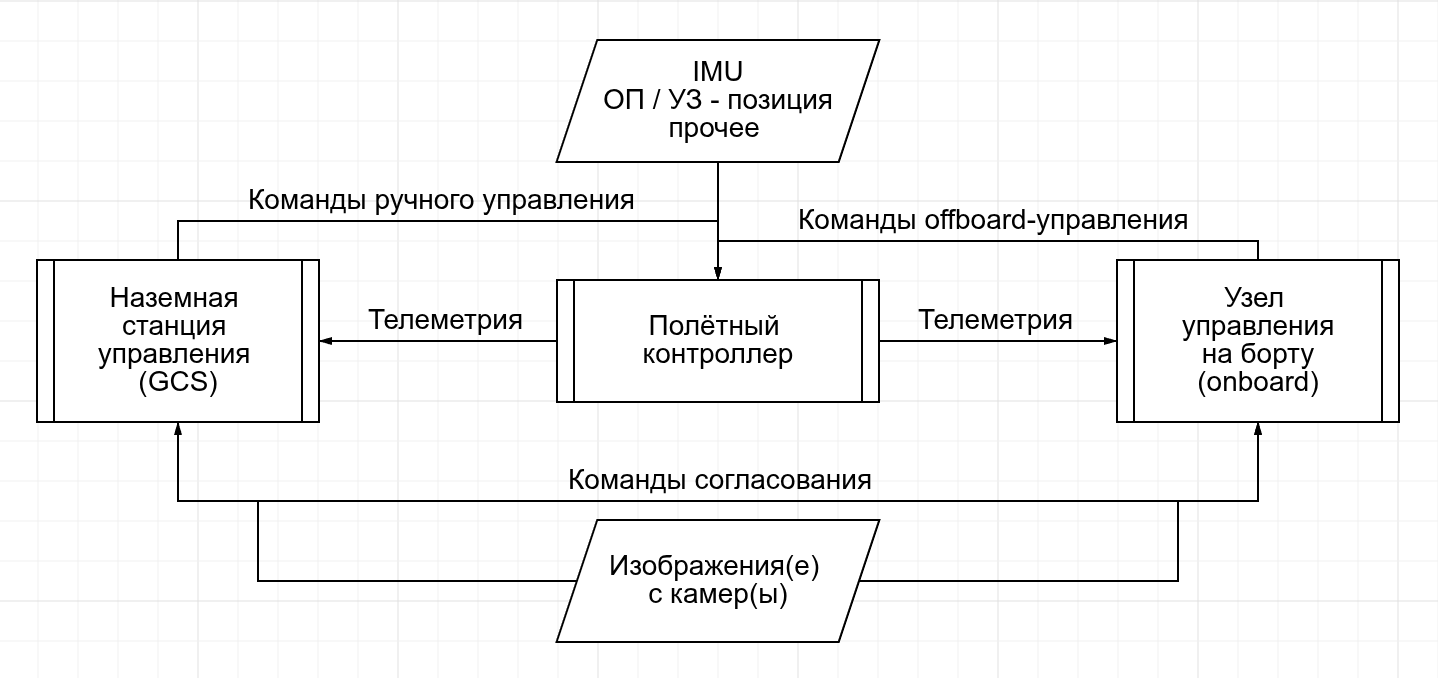
\includegraphics[width=\linewidth]{scheme.png}
  \caption{Схема управления полётом}
  \label{fig:control_scheme}
\end{figure}
Предполагается одновременное наличие двух согласованных источников управления полётом: GCS (Ground Control Station, наземная станция управления) и onboard (котроллер на борту). На рискунке~\ref{fig:control_scheme} изображёна схема подключения дрона к элементам управления полётом. 

\begin{itemize}
  \item GCS отвечает за управления дроном в ручном режиме, управление миссией (формирование, запуск, остановка, пауза и т.д.), предоставление пользовательского интерфейса оператору. 
  \item Onboard -- контроллер управления дроном в режиме миссии. На основании компьютерного зрения и положения дрона определяет следующее его действие, тем самым выполняя задание.
\end{itemize}

\textit{Примечание}. Под ОП/УЗ-позиционированием дрона подразумевается определние мировых координат БАС посредством оптического потока (OpticalFlow, OF, ОП) или ультра-звуковых маяков (УЗ).

\section{Описание миссии}

\subsection{Логика полёта}
Одна итерация полётной миссии дрона состоит из следующих шагов:
\begin{itemize}
  \item \textbf{Старт полёта}: взлёт и занимание исходного положения над ``складом''. Автоматический режим может включиться со стата или с занятого вручную положения в воздухе.
  \item \textbf{Определение цели}: в зафискированном положении дрон должен обнаружить груз-модель (предполагается использовать относительное позиционирование груза через AptilTag).
  \item \textbf{Захват цели}: дрон должен занять положение над целью и выполнить её захват.
  \item \textbf{Полёт до точки назначения}: дрон должен по заранее согласованному маршруту прибыть в точку назначения и занять исходное положение над ней.
  \item \textbf{Определение точки установки груза}: средствами компьютерного зрения дрон должен определить точку установки/сброса груза.
  \item \textbf{Установка груза}: занять необходимое положение и сбросить груз.
  \item \textbf{Возврат на исходное или завершение миссии}.
\end{itemize}

\subsection{Допуски и координаты}
\textit{Будут определены в последующих редакциях}

\subsection{Нештатные или аварийные ситуации}
\begin{itemize}
  \item \textbf{Обрыв соединения GCS -- onboard при наличии соединения GCS -- дрон}: GCS переводит дрон в режим удержания текущего положения, отправляет дрону команду игнорирования ввода onboard, пытается отправить команду аварийного прерывания исполнения миссии и передаёт управление оператору.
  \item \textbf{Обрыв соединения GCS -- onboard при наличии соединения onboard -- дрон}: onboard прерывает исполнение миссии, совершает аварийную посадку и выключает двигатели.
  \item \textbf{Обрыв соединения дрон -- управление}: при потери полётным контроллером сигналов от двух источников дрон должен соверщить немедленную аварийную посадку (при возможности на посадочную площадку).
  \item \textbf{Превышение скорости}: при преодоление заранее заданного предела скорости дрона и(или) угла наклона должен выйти в состояния удержания текущей позиции.
  \item \textbf{Хаотичное движение}: аварийное выключение двигателей. Определение хаотического движения будет дано в последующих редакциях.
\end{itemize}

\end{document}